\usetikzlibrary{calc, arrows.meta, intersections, patterns, positioning, shapes.misc, fadings, through,decorations.pathreplacing}

\begin{figure}[!h]
\centering
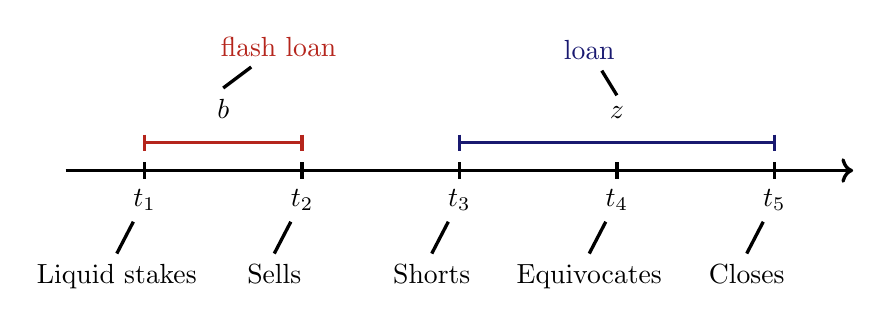
\begin{tikzpicture}[very thick, black]

\coordinate (O) at (-1,0); % Origin
\coordinate (P1) at (0, 0);
\coordinate (P2) at (2, 0);
\coordinate (P3) at (4, 0);
\coordinate (P4) at (6, 0);
\coordinate (P5) at (8, 0);
\coordinate (F) at (9,0); %End


%% Timeline
\draw[->] (O) -- (F);

%% Ticks
\foreach \x in {0,2,...,8}
\draw (\x cm,3pt) -- (\x cm,-3pt);


%% t_0
\draw (P1) node[below=3pt](T1) {$t_1$} ;
\node[below=30pt,xshift=-10pt](D1) at (P1) {%
	Liquid stakes};
\draw (T1) --  (D1.north);

%% t_1
\draw (P2) node[below=3pt](T2) {$t_2$} ;
\node[below=30pt,xshift=-10pt](D2) at (P2) {%
	Sells};
\draw (T2) --  (D2.north);

%% t_2
\draw (P3) node[below=3pt](T3) {$t_3$} ;
\node[below=30pt,xshift=-10pt](D3) at (P3) {%
	Shorts};
\draw (T3) --  (D3.north);

%% t_3
\draw (P4) node[below=3pt](T4) {$t_4$} ;
\node[below=30pt,xshift=-10pt](D4) at (P4) {%
  Equivocates};
\draw (T4) --  (D4.north);

%% t_4
\draw (P5) node[below=3pt](T5) {$t_5$} ;
\node[below=30pt,xshift=-10pt](D5) at (P5) {%
  Closes};
\draw (T5) --  (D5.north);


%% Loans
\coordinate[above=10pt] (R1) at (P1);
\coordinate[above=10pt] (R2) at (P2);
\coordinate[above=10pt] (R3) at (P3);
\coordinate[above=10pt] (R5) at (P5);

\draw[color=BrickRed] ($(R1) + (0,3pt)$) -- ($(R1) + (0,-3pt)$);
\draw[color=BrickRed] ($(R2) + (0,3pt)$) -- ($(R2) + (0,-3pt)$);
\draw[color=BrickRed] (R1) -- (R2) node[color=black,midway, above=5pt](L1) {$b$ {\tiny \asset}};
\node[text=BrickRed,above=15pt,xshift=20pt](LD2) at (L1) {%
	flash loan};
\draw (LD2) --  (L1.north);

\draw[color=MidnightBlue] ($(R3) + (0,3pt)$) -- ($(R3) + (0,-3pt)$);
\draw[color=MidnightBlue] ($(R5) + (0,3pt)$) -- ($(R5) + (0,-3pt)$);
\draw[color=MidnightBlue] (R3) -- (R5) node[color=black,midway, above=5pt](L2) {$z$ {\tiny \stasset}};
\node[text=MidnightBlue,above=15pt,xshift=-10pt](LD3) at (L2) {%
	loan};
\draw (LD3) --  (L2.north);

\end{tikzpicture}

\caption{Timeline of the attack.}
\label{fig:timeline}
\end{figure}